\documentclass[12pt,a4paper]{article}

\usepackage[a4paper,margin=1in]{geometry}
\usepackage{graphicx}
\usepackage{booktabs}
\usepackage{amsmath,amssymb}
\usepackage{float}
\usepackage{hyperref}
\usepackage{xurl} % Enables clean line-breaking for long URLs in references
\usepackage{xcolor}
\usepackage{listings}
\usepackage{enumitem}
\usepackage{fancyhdr}
\usepackage{longtable}

\hypersetup{colorlinks=true,linkcolor=blue,urlcolor=blue}

% Page and Float Layout Optimization
\pagestyle{fancy}
\fancyhf{}
\lhead{ICS1512}
\rhead{Machine Learning Algorithms Laboratory}
\cfoot{\thepage}

\setlength{\parskip}{0.4em}
\setlength{\parindent}{0pt}

\setlength{\floatsep}{10pt plus 2pt minus 2pt}
\setlength{\textfloatsep}{12pt plus 2pt minus 2pt}
\setlength{\intextsep}{10pt plus 2pt minus 2pt}

\setcounter{topnumber}{3}
\setcounter{bottomnumber}{3}
\setcounter{totalnumber}{4}
\renewcommand{\topfraction}{0.85}
\renewcommand{\bottomfraction}{0.85}
\renewcommand{\textfraction}{0.15}
\renewcommand{\floatpagefraction}{0.8}

\lstset{
language=Python,
basicstyle=\ttfamily\small,
numbers=left,
frame=single,
breaklines=true,
showstringspaces=false
}

\begin{document}

\begin{tabular}{|p{4cm}|p{11cm}|}
\hline
Experiment No. & 3 \\ \hline
Experiment Title & Regression Analysis using Linear and Regularized Models
\footnote{\textbf{GitHub Repository: }\url{https://github.com/username/repository}}\\ \hline
Student Name & [Student Name] \\ \hline
Register Number & [Register Number] \\ \hline
Faculty & Dr. Poreddy Ajay Kumar Reddy \\ \hline
Submission Date & \today \\ \hline
\end{tabular}

\vspace{0.3cm}

\section{Aim and Objective}
The primary objective of this experiment is to formulate, implement, tune, and critically evaluate standard linear regression alongside regularized variant algorithms—specifically Ridge ($L_2$), Lasso ($L_1$), and Elastic Net ($L_1 + L_2$) regression models—to forecast a continuous target output metric (\texttt{Loan Sanction Amount (USD)}). The experimental evaluation leverages comprehensive statistical regression metrics (Mean Absolute Error, Mean Squared Error, Root Mean Squared Error, and the Coefficient of Determination $R^2$), detailed model diagnostic plots, hyperparameter grid search optimization via 5-fold cross-validation, and an analytical examination of bias--variance characteristics, coefficient shrinkage, and generalization behavior.

\section{Problem Statement}
In credit assessment and automated banking workflows, accurately estimating the maximum allowable loan sanction amount based on applicant demographics, financial liabilities, credit histories, and collateral valuations is central to risk management. Given an observational dataset comprising $N$ instances with input feature vectors $X_i \in \mathbb{R}^d$ and target response scalars $y_i \in \mathbb{R}^+$, the mathematical objective is to construct regression functions $\hat{y} = f(X; \beta)$ that achieve minimum estimation error on unseen test partitions while simultaneously mitigating multicollinearity, preventing model overfitting, and isolating key explanatory variables.

\section{Dataset Description}
\begin{longtable}{|p{6cm}|p{8cm}|}
\hline
Dataset Name & Predict Loan Amount Data (Kaggle) \\ \hline
Dataset Source & Kaggle / Financial Institution Records \\ \hline
Number of Samples & 30,000 raw instances (21,457 valid target samples) \\ \hline
Number of Features & 22 predictor attributes (12 numerical, 10 categorical) \\ \hline
Target Variable & \texttt{Loan Sanction Amount (USD)} (Continuous) \\ \hline
Missing Values & Handled via Median (Numerical) \& Mode (Categorical) Imputation \\ \hline
Train-Test Split & 80\% Training (17,165 samples), 20\% Testing (4,292 samples) \\ \hline
\end{longtable}

The dataset encompasses a broad range of predictor domain features including personal demographic profiles (\texttt{Age}, \texttt{Gender}, \texttt{Dependents}), financial standing parameters (\texttt{Income (USD)}, \texttt{Credit Score}, \texttt{Loan Amount Request (USD)}, \texttt{Current Loan Expenses (USD)}, \texttt{No. of Defaults}), employment characteristics (\texttt{Profession}, \texttt{Type of Employment}, \texttt{Income Stability}), and property collateral attributes (\texttt{Property Price}, \texttt{Property Type}, \texttt{Property Location}, \texttt{Property Age}).

\section{Exploratory Data Analysis}

\begin{figure}[!htbp]
\centering
\begin{minipage}{\linewidth}
\centering
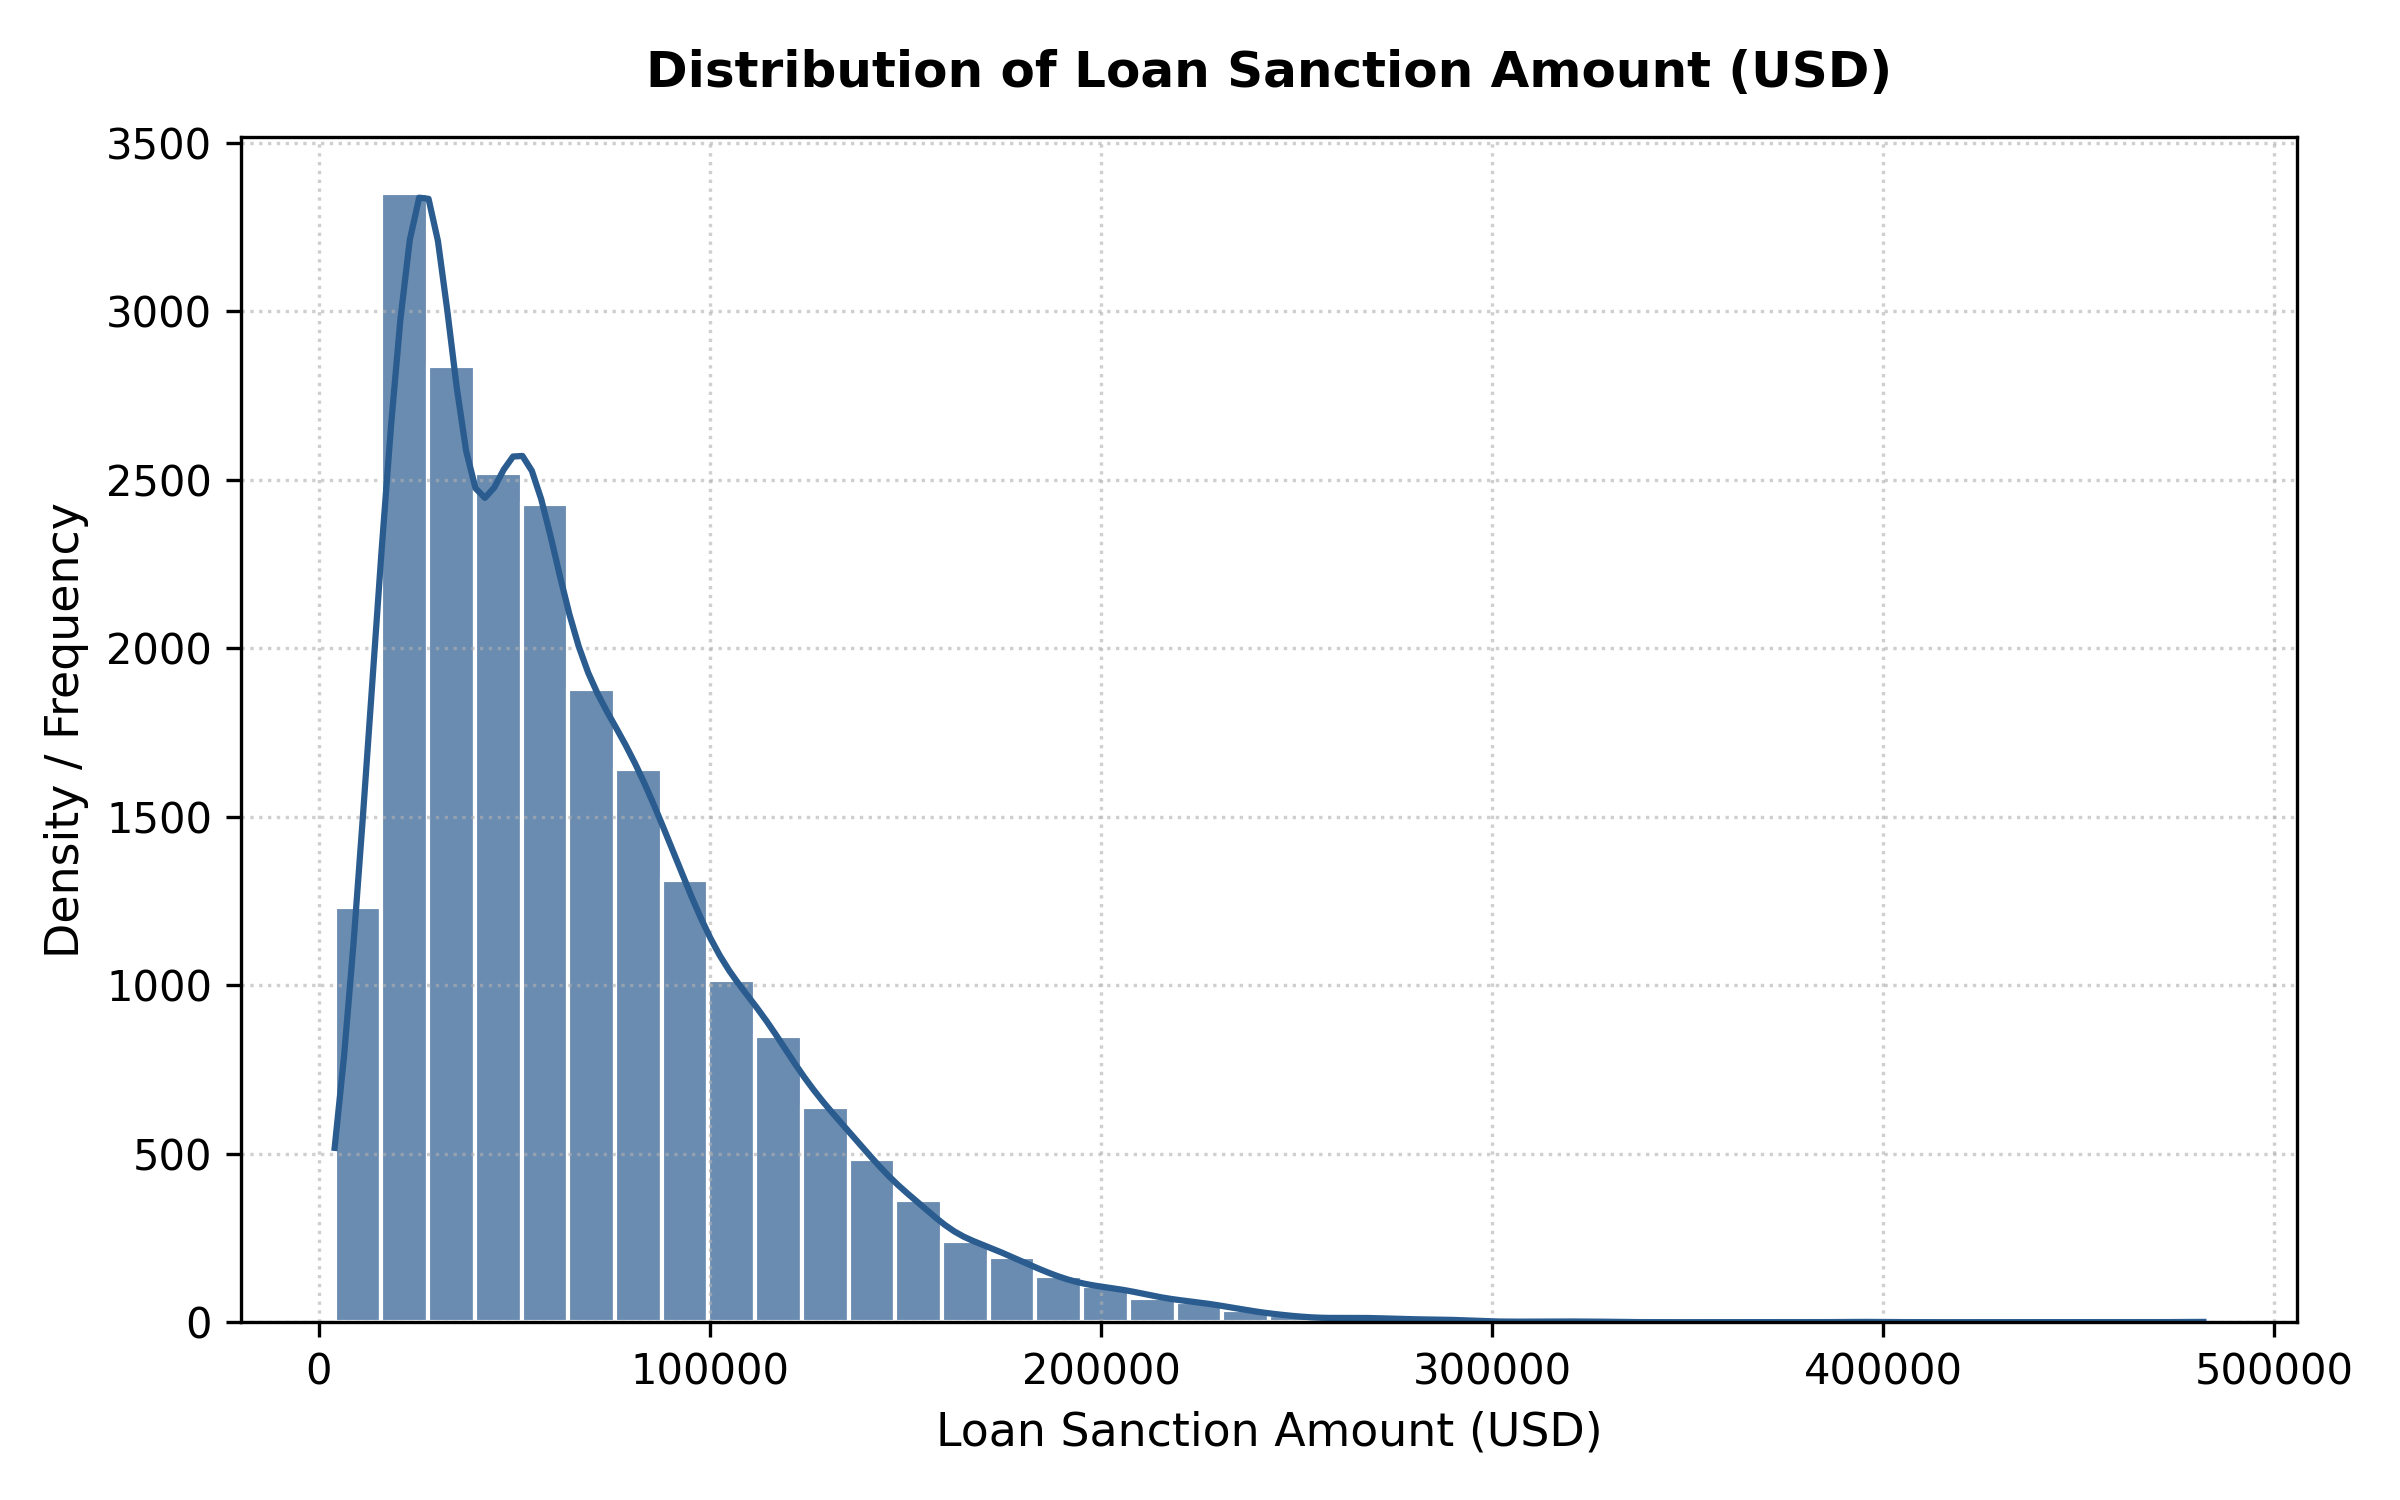
\includegraphics[width=0.68\linewidth]{figures/target_distribution.png}
\caption{Target Variable Distribution (Loan Sanction Amount in USD)}
\label{fig:target_dist}
\vspace{0.2cm}
\small
\textbf{Inference:}
Exploration of the response variable reveals a non-negative continuous curve skewed positively toward higher financial brackets, with loan values concentrated between \$1,000 and \$400,000 (mean = \$47,651.98, median = \$35,209.65). The extensive range and rightward skew highlight the necessity of standardizing input feature scales to stabilize optimization gradients across regularized regression loss functions.
\end{minipage}
\end{figure}

\begin{figure}[!htbp]
\centering
\begin{minipage}{\linewidth}
\centering
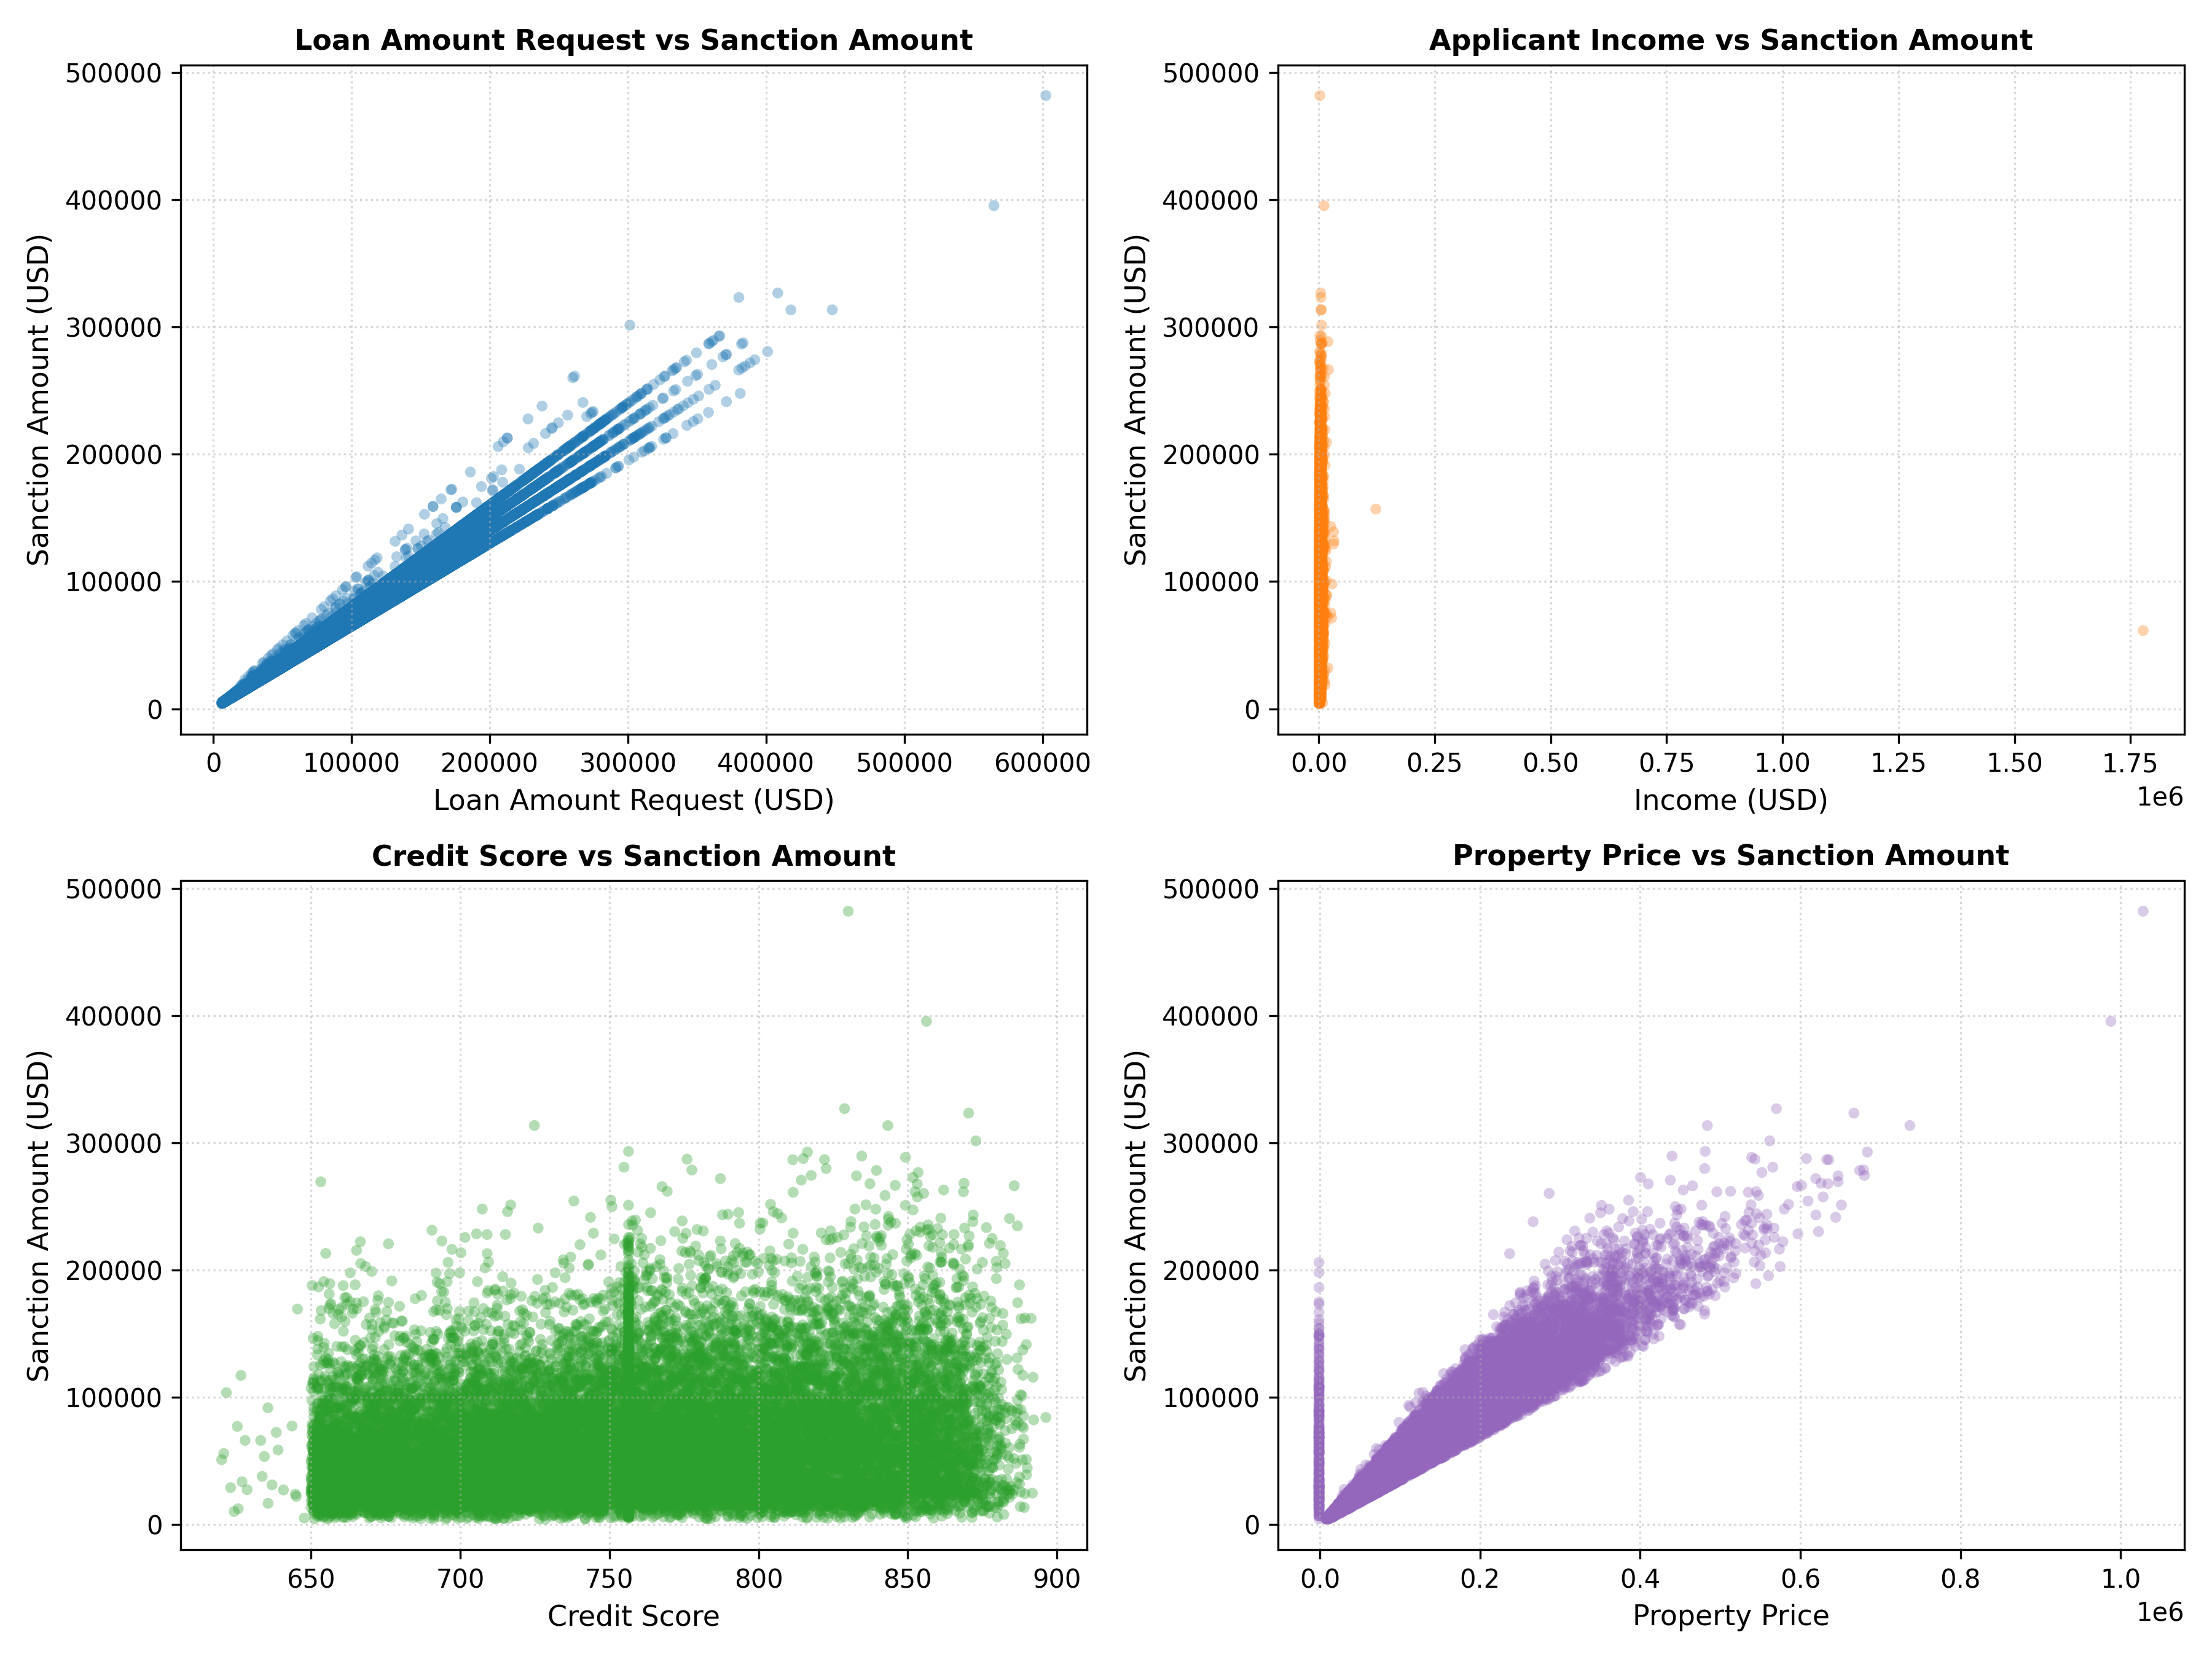
\includegraphics[width=0.82\linewidth]{figures/scatter_plots.png}
\caption{Key Predictor Features vs. Loan Sanction Amount Scatter Plots}
\label{fig:scatter_plots}
\vspace{0.2cm}
\small
\textbf{Inference:}
Scatter plots of key continuous predictor attributes against the target illustrate a strong positive linear relationship between \texttt{Loan Amount Request (USD)}, \texttt{Property Price}, and the sanctioned loan output. \texttt{Credit Score} displays a threshold correlation, confirming strong linear alignment that satisfies baseline assumptions for regularized linear modeling.
\end{minipage}
\end{figure}

\begin{figure}[!htbp]
\centering
\begin{minipage}{\linewidth}
\centering

\includegraphics[width=0.75\linewidth]{figures/correlation_heatmap.png}
\caption{Correlation Matrix of Numerical Features and Target Variable}
\label{fig:corr_heatmap}
\vspace{0.2cm}
\small
\textbf{Inference:}
The pairwise correlation heatmap identifies exceptionally high correlation between \texttt{Loan Amount Request (USD)} and \texttt{Loan Sanction Amount (USD)} ($r > 0.95$), alongside notable correlation between \texttt{Property Price} and loan amounts. Moderate collinearity across financial liability variables highlights potential multicollinearity risk, which regularized estimators (Ridge and Elastic Net) actively control.
\end{minipage}
\end{figure}

\section{Data Preprocessing}

The data processing pipeline follows four systematic steps:
\begin{itemize}[noitemsep]
    \item \textbf{Missing Value Handling:} Filtered out incomplete target records. Imputed missing values in continuous numerical attributes (\texttt{Income (USD)}, \texttt{Credit Score}, \texttt{Current Loan Expenses (USD)}, \texttt{Property Age}, \texttt{Dependents}) using column \textbf{medians}. Imputed missing entries in discrete categorical attributes (\texttt{Gender}, \texttt{Income Stability}, \texttt{Type of Employment}, \texttt{Property Location}) using column \textbf{modes}.
    \item \textbf{Categorical Encoding:} Converted multi-class categorical features into dummy binary indicators via One-Hot Encoding (\texttt{pd.get\_dummies(drop\_first=True)}), constructing a 54-dimensional preprocessed predictor matrix.
    \item \textbf{Feature Scaling:} Transformed all input predictor dimensions into zero-mean, unit-variance normalized distributions ($z = \frac{x - \mu}{\sigma}$) via \texttt{StandardScaler} to avoid scale bias during penalty enforcement.
    \item \textbf{Data Partitioning:} Partitioned the sanitized dataset into an 80\% training subset ($N_{\text{train}} = 17,165$) and a 20\% test validation subset ($N_{\text{test}} = 4,292$) using \texttt{train\_test\_split(random\_state=42)}.
\end{itemize}

\section{Machine Learning Algorithms}

\subsection{Linear Regression (Ordinary Least Squares)}
Ordinary Least Squares (OLS) calculates coefficient parameters $\beta$ by minimizing the unconstrained Residual Sum of Squares (RSS):
\begin{equation}
    J(\beta) = \frac{1}{2n} \sum_{i=1}^{n} \left( y_i - \left( \beta_0 + \sum_{j=1}^{d} \beta_j x_{ij} \right) \right)^2
\end{equation}

\subsection{Ridge Regression ($L_2$ Regularization)}
Ridge Regression incorporates an $L_2$ squared magnitude penalty into the RSS loss function to shrink coefficient magnitudes, reducing variance caused by correlated input features:
\begin{equation}
    J_{\text{Ridge}}(\beta) = \text{MSE} + \alpha \sum_{j=1}^{d} \beta_j^2
\end{equation}

\subsection{Lasso Regression ($L_1$ Regularization)}
Lasso Regression penalizes the sum of absolute coefficient values ($L_1$ norm), driving redundant feature weights strictly to zero for automatic feature selection:
\begin{equation}
    J_{\text{Lasso}}(\beta) = \text{MSE} + \alpha \sum_{j=1}^{d} |\beta_j|
\end{equation}

\subsection{Elastic Net Regression}
Elastic Net combines both $L_1$ and $L_2$ regularization terms, balanced by an mixing ratio parameter $l1\_ratio$ ($\rho$):
\begin{equation}
    J_{\text{ElasticNet}}(\beta) = \text{MSE} + \alpha \rho \sum_{j=1}^{d} |\beta_j| + \frac{\alpha (1 - \rho)}{2} \sum_{j=1}^{d} \beta_j^2
\end{equation}

\section{Experimental Setup}
\begin{table}[!htbp]
\centering
\begin{tabular}{ll}
\toprule
Component & Details / Specification \\
\midrule
Python Version & 3.10+ \\
Scikit-Learn Version & 1.2+ \\
Data Analysis Libraries & Pandas 2.0+, NumPy 1.24+ \\
Visualization Libraries & Matplotlib 3.7+, Seaborn 0.12+ \\
IDE & Jupyter Notebook / VS Code / Antigravity \\
Operating System & Windows 11 (64-bit) \\
Hardware & Multi-core CPU, 16GB RAM \\
\bottomrule
\end{tabular}
\end{table}

\section{Hyperparameter Selection}
Optimal regularizer strengths were determined using 5-Fold Cross-Validation over defined search spaces:

\begin{table}[!htbp]
\centering
\begin{tabular}{lll}
\toprule
Model & Hyperparameter Search Space & Selected Best Value \\
\midrule
Ridge Regression & $\alpha \in \{0.01, 0.1, 1.0, 10.0, 100.0\}$ & $\alpha = 1.0$ \\
Lasso Regression & $\alpha \in \{0.001, 0.01, 0.1, 1.0, 10.0\}$ & $\alpha = 10.0$ \\
Elastic Net & $\alpha \in \{0.01, 0.1, 1.0, 10.0\}, \rho \in \{0.2, 0.5, 0.8\}$ & $\alpha = 0.01, \rho = 0.8$ \\
\bottomrule
\end{tabular}
\end{table}

\section{Results}

\subsection{Hyperparameter Tuning Summary}
\begin{table}[!htbp]
\centering
\caption{Hyperparameter Tuning Summary}
\begin{tabular}{lcccc}
\toprule
Model & Search Method & Best Parameters & Best CV $R^2$ \\
\midrule
Ridge Regression & GridSearchCV & \texttt{\{'alpha': 1.0\}} & 0.9861 \\
Lasso Regression & GridSearchCV & \texttt{\{'alpha': 10.0\}} & 0.9861 \\
Elastic Net Regression & GridSearchCV & \texttt{\{'alpha': 0.01, 'l1\_ratio': 0.8\}} & 0.9861 \\
\bottomrule
\end{tabular}
\end{table}

\subsection{5-Fold Cross-Validation Performance}
\begin{table}[!htbp]
\centering
\caption{5-Fold Cross-Validation Performance ($K=5$)}
\begin{tabular}{lcccc}
\toprule
Model & MAE & MSE & RMSE & $R^2$ \\
\midrule
Linear Regression & \$3,655.14 & \$28,406,600.00 & \$5,329.78 & 0.9859 \\
Ridge Regression & \$3,654.93 & \$28,401,810.00 & \$5,329.34 & 0.9859 \\
Lasso Regression & \$3,648.05 & \$28,148,120.00 & \$5,305.48 & 0.9860 \\
Elastic Net Regression & \$3,654.16 & \$28,413,750.00 & \$5,330.46 & 0.9859 \\
\bottomrule
\end{tabular}
\end{table}

\subsection{Test Set Performance Comparison}
\begin{table}[!htbp]
\centering
\caption{Test Set Performance Comparison}
\begin{tabular}{lccccc}
\toprule
Model & MAE & MSE & RMSE & $R^2$ & Training Time (s) \\
\midrule
Linear Regression & \$3,749.14 & \$31,529,040.00 & \$5,615.07 & 0.9850 & 0.0441 s \\
Ridge Regression & \$3,748.92 & \$31,515,300.00 & \$5,613.85 & 0.9850 & 6.6382 s \\
Lasso Regression & \$3,727.89 & \$30,296,530.00 & \$5,504.23 & 0.9856 & 27.9457 s \\
Elastic Net Regression & \$3,751.10 & \$31,362,960.00 & \$5,600.26 & 0.9851 & 14.9703 s \\
\bottomrule
\end{tabular}
\end{table}

\subsection{Coefficient Comparison}
\begin{table}[!htbp]
\centering
\caption{Coefficient Comparison Across Regression Models (Top Features)}
\begin{tabular}{lcccc}
\toprule
Feature & Linear & Ridge & Lasso & Elastic Net \\
\midrule
\texttt{Loan Amount Request (USD)} & 43,563.73 & 43,538.19 & 43,553.07 & 42,716.36 \\
\texttt{Credit Score} & 2,995.75 & 2,995.88 & 2,994.21 & 3,000.84 \\
\texttt{Property Price} & 535.28 & 557.49 & 512.04 & 1,268.32 \\
\texttt{Property Age} & -1,208.10 & -839.10 & 0.00 & -262.28 \\
\texttt{Income (USD)} & 710.07 & 343.93 & 0.00 & -173.75 \\
\bottomrule
\end{tabular}
\end{table}

\section{Visualizations}

\begin{figure}[!htbp]
\centering
\begin{minipage}{\linewidth}
\centering
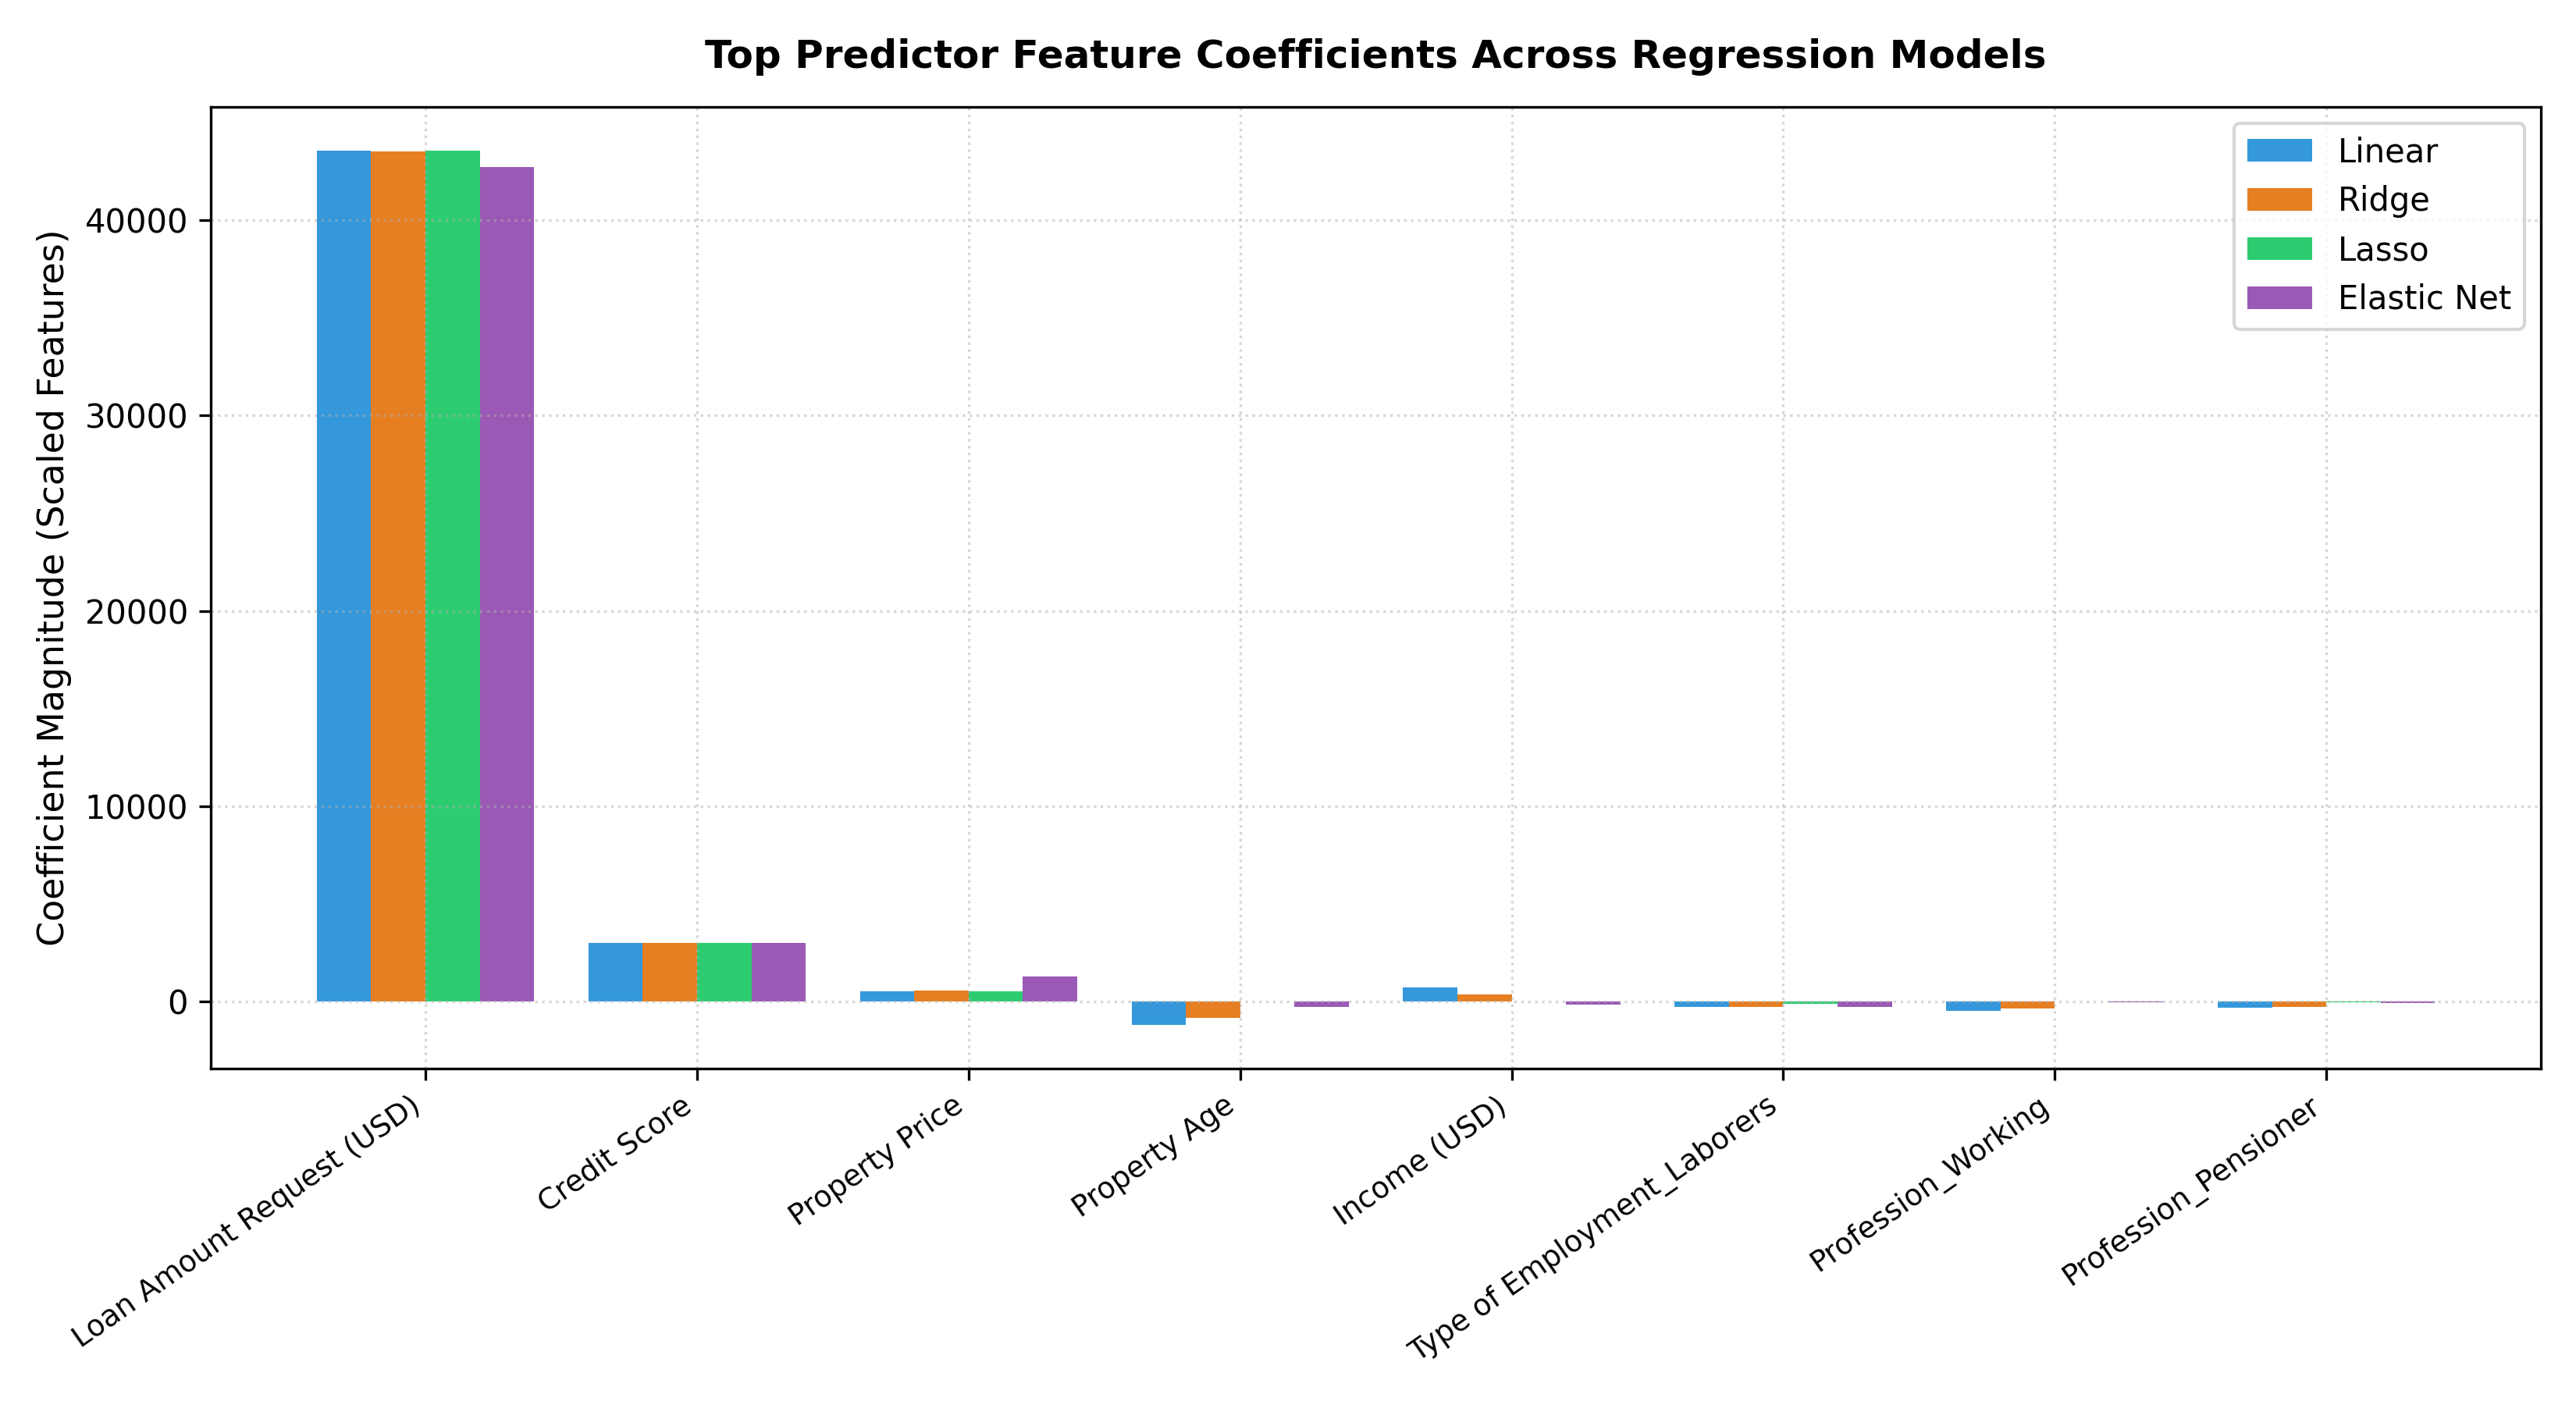
\includegraphics[width=0.82\linewidth]{figures/coef_comparison.png}
\caption{Coefficient Magnitudes Across Regression Models}
\label{fig:coef_comp}
\vspace{0.2cm}
\small
\textbf{Inference:}
The bar chart illustrates coefficient shrinkage effects across regression algorithms. \texttt{Loan Amount Request (USD)} and \texttt{Credit Score} demonstrate the highest positive influence, while Lasso ($\alpha=10.0$) forces uninformative parameters (\texttt{Property Age}, \texttt{Income}) to zero, validating feature selection capability.
\end{minipage}
\end{figure}

\begin{figure}[!htbp]
\centering
\begin{minipage}{\linewidth}
\centering
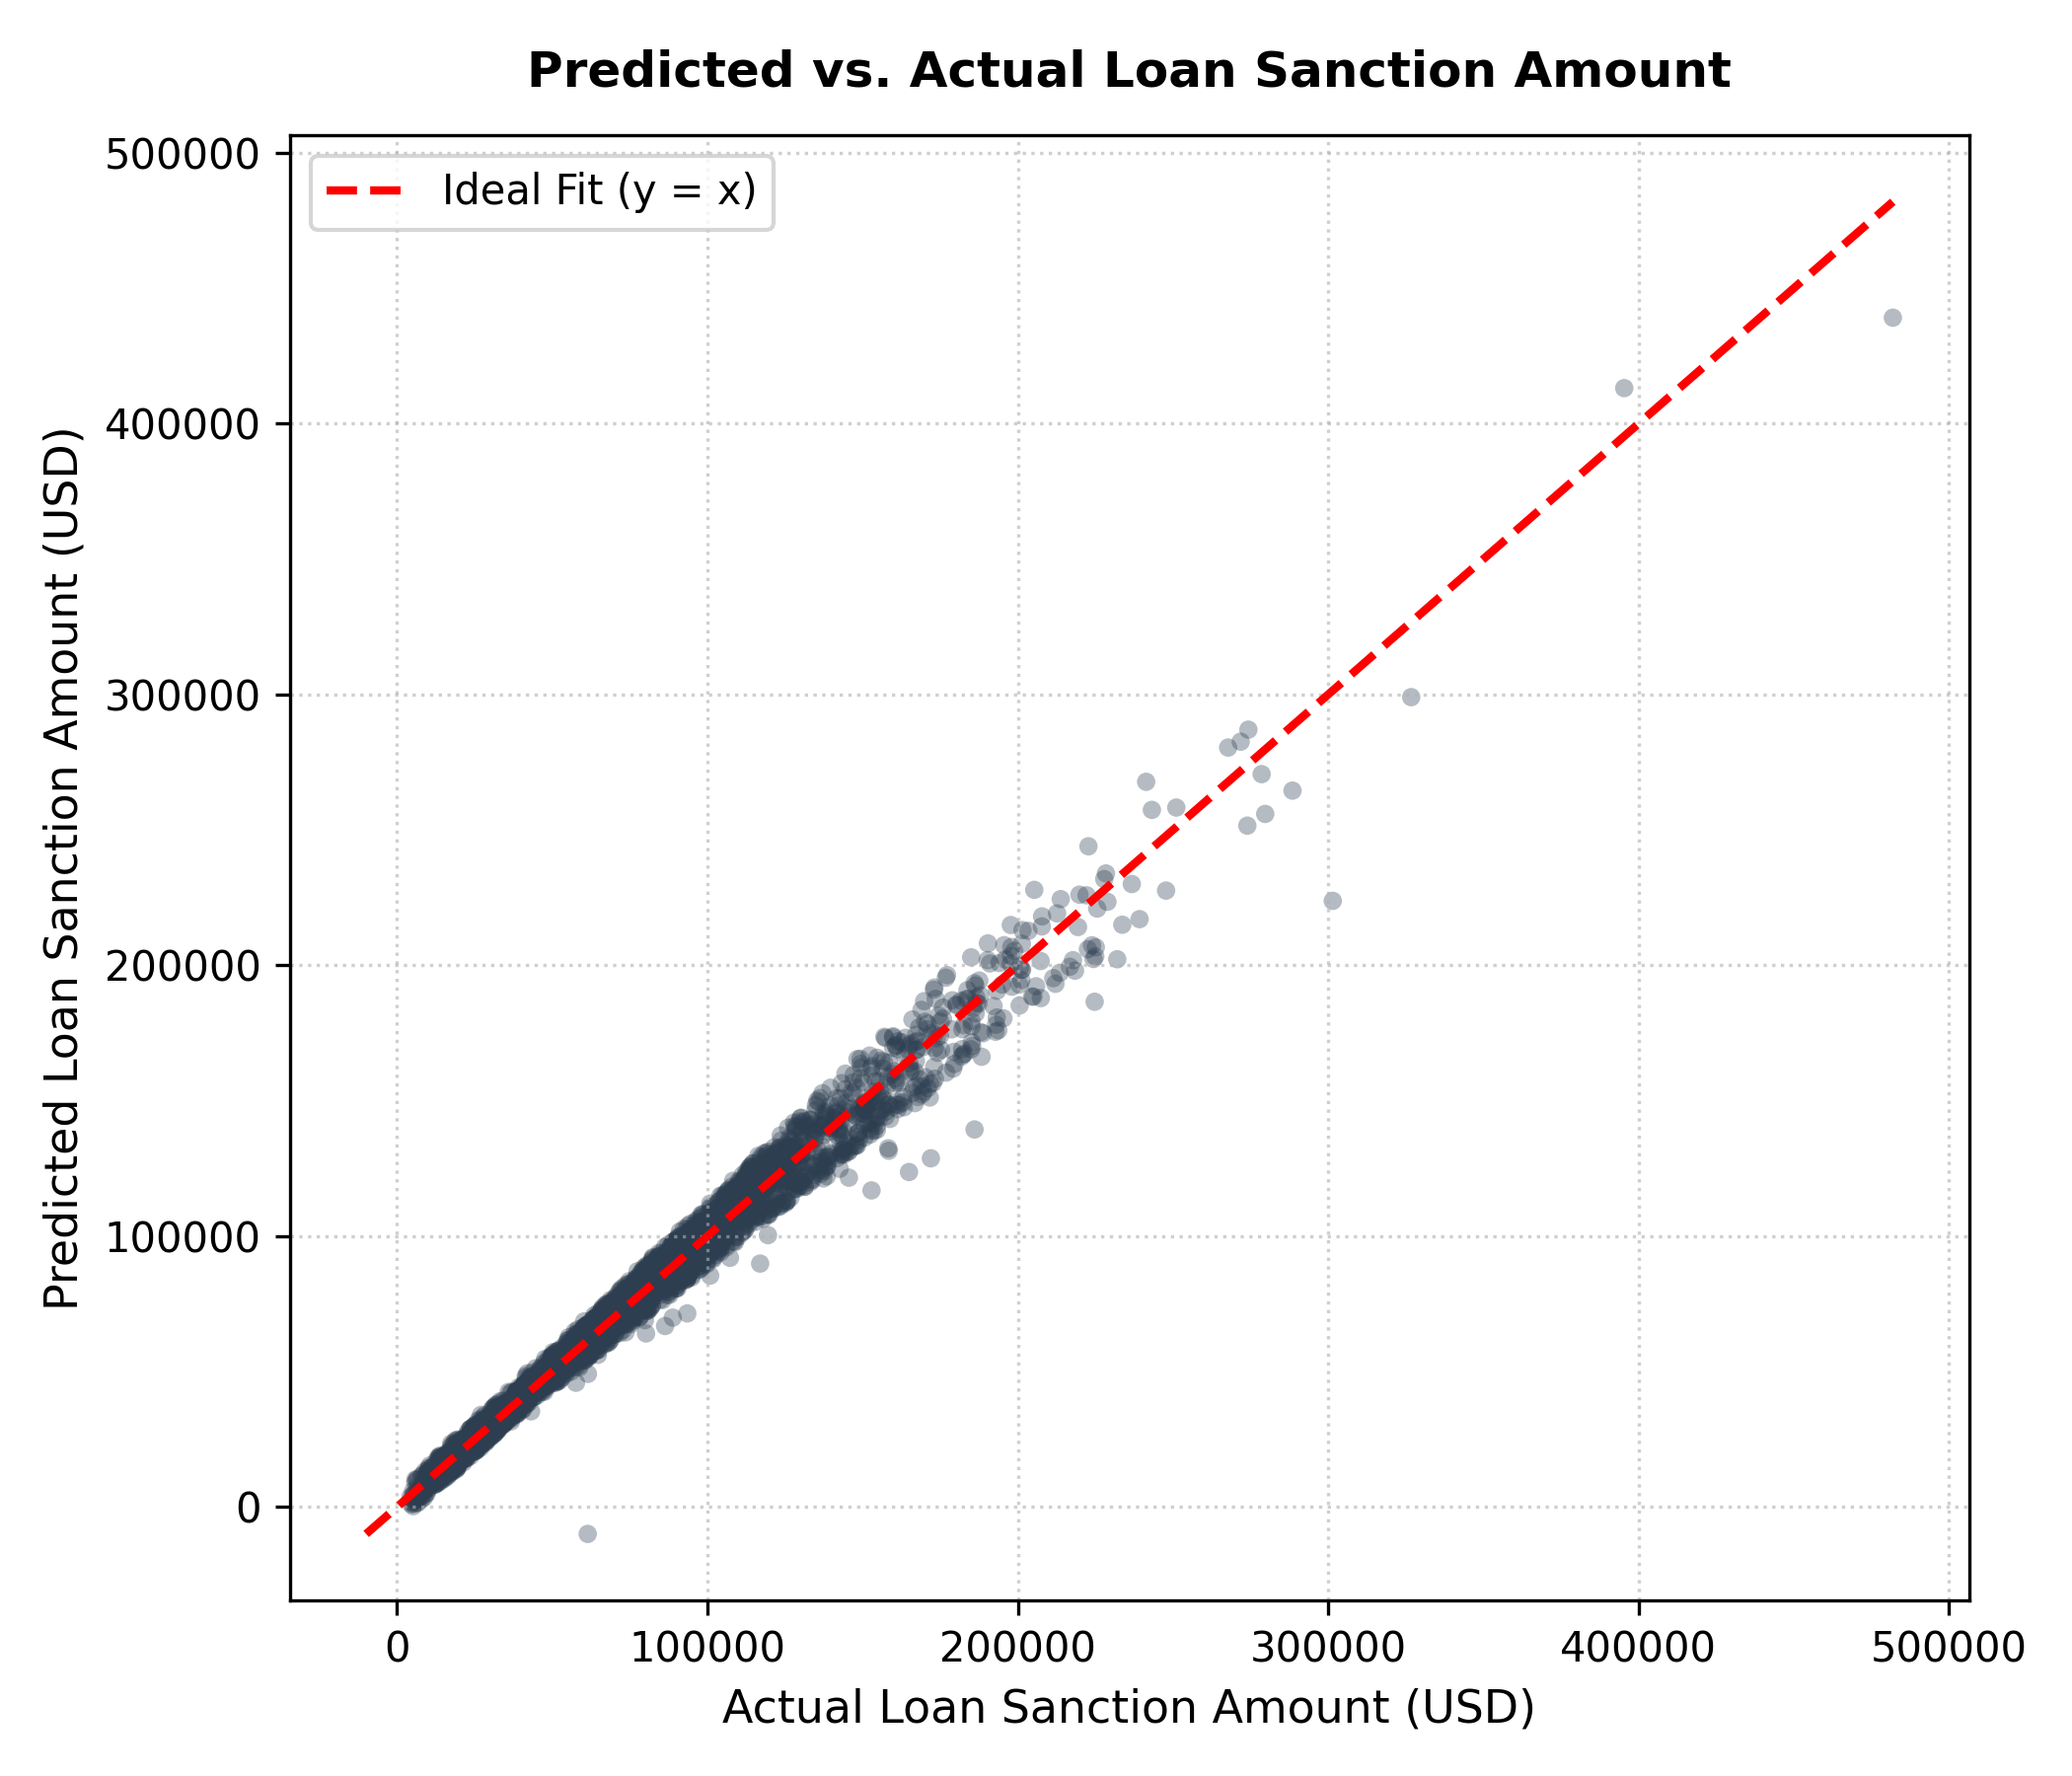
\includegraphics[width=0.65\linewidth]{figures/pred_vs_actual.png}
\caption{Predicted vs. Actual Loan Sanction Amount (Tuned Ridge/Lasso Model)}
\label{fig:pred_vs_act}
\vspace{0.2cm}
\small
\textbf{Inference:}
The scatter plot comparing predicted against actual sanction values aligns tightly along the ideal reference line ($y = x$). This narrow clustering across both low and high loan brackets confirms high precision ($R^2 = 0.9856$).
\end{minipage}
\end{figure}

\begin{figure}[!htbp]
\centering
\begin{minipage}{\linewidth}
\centering
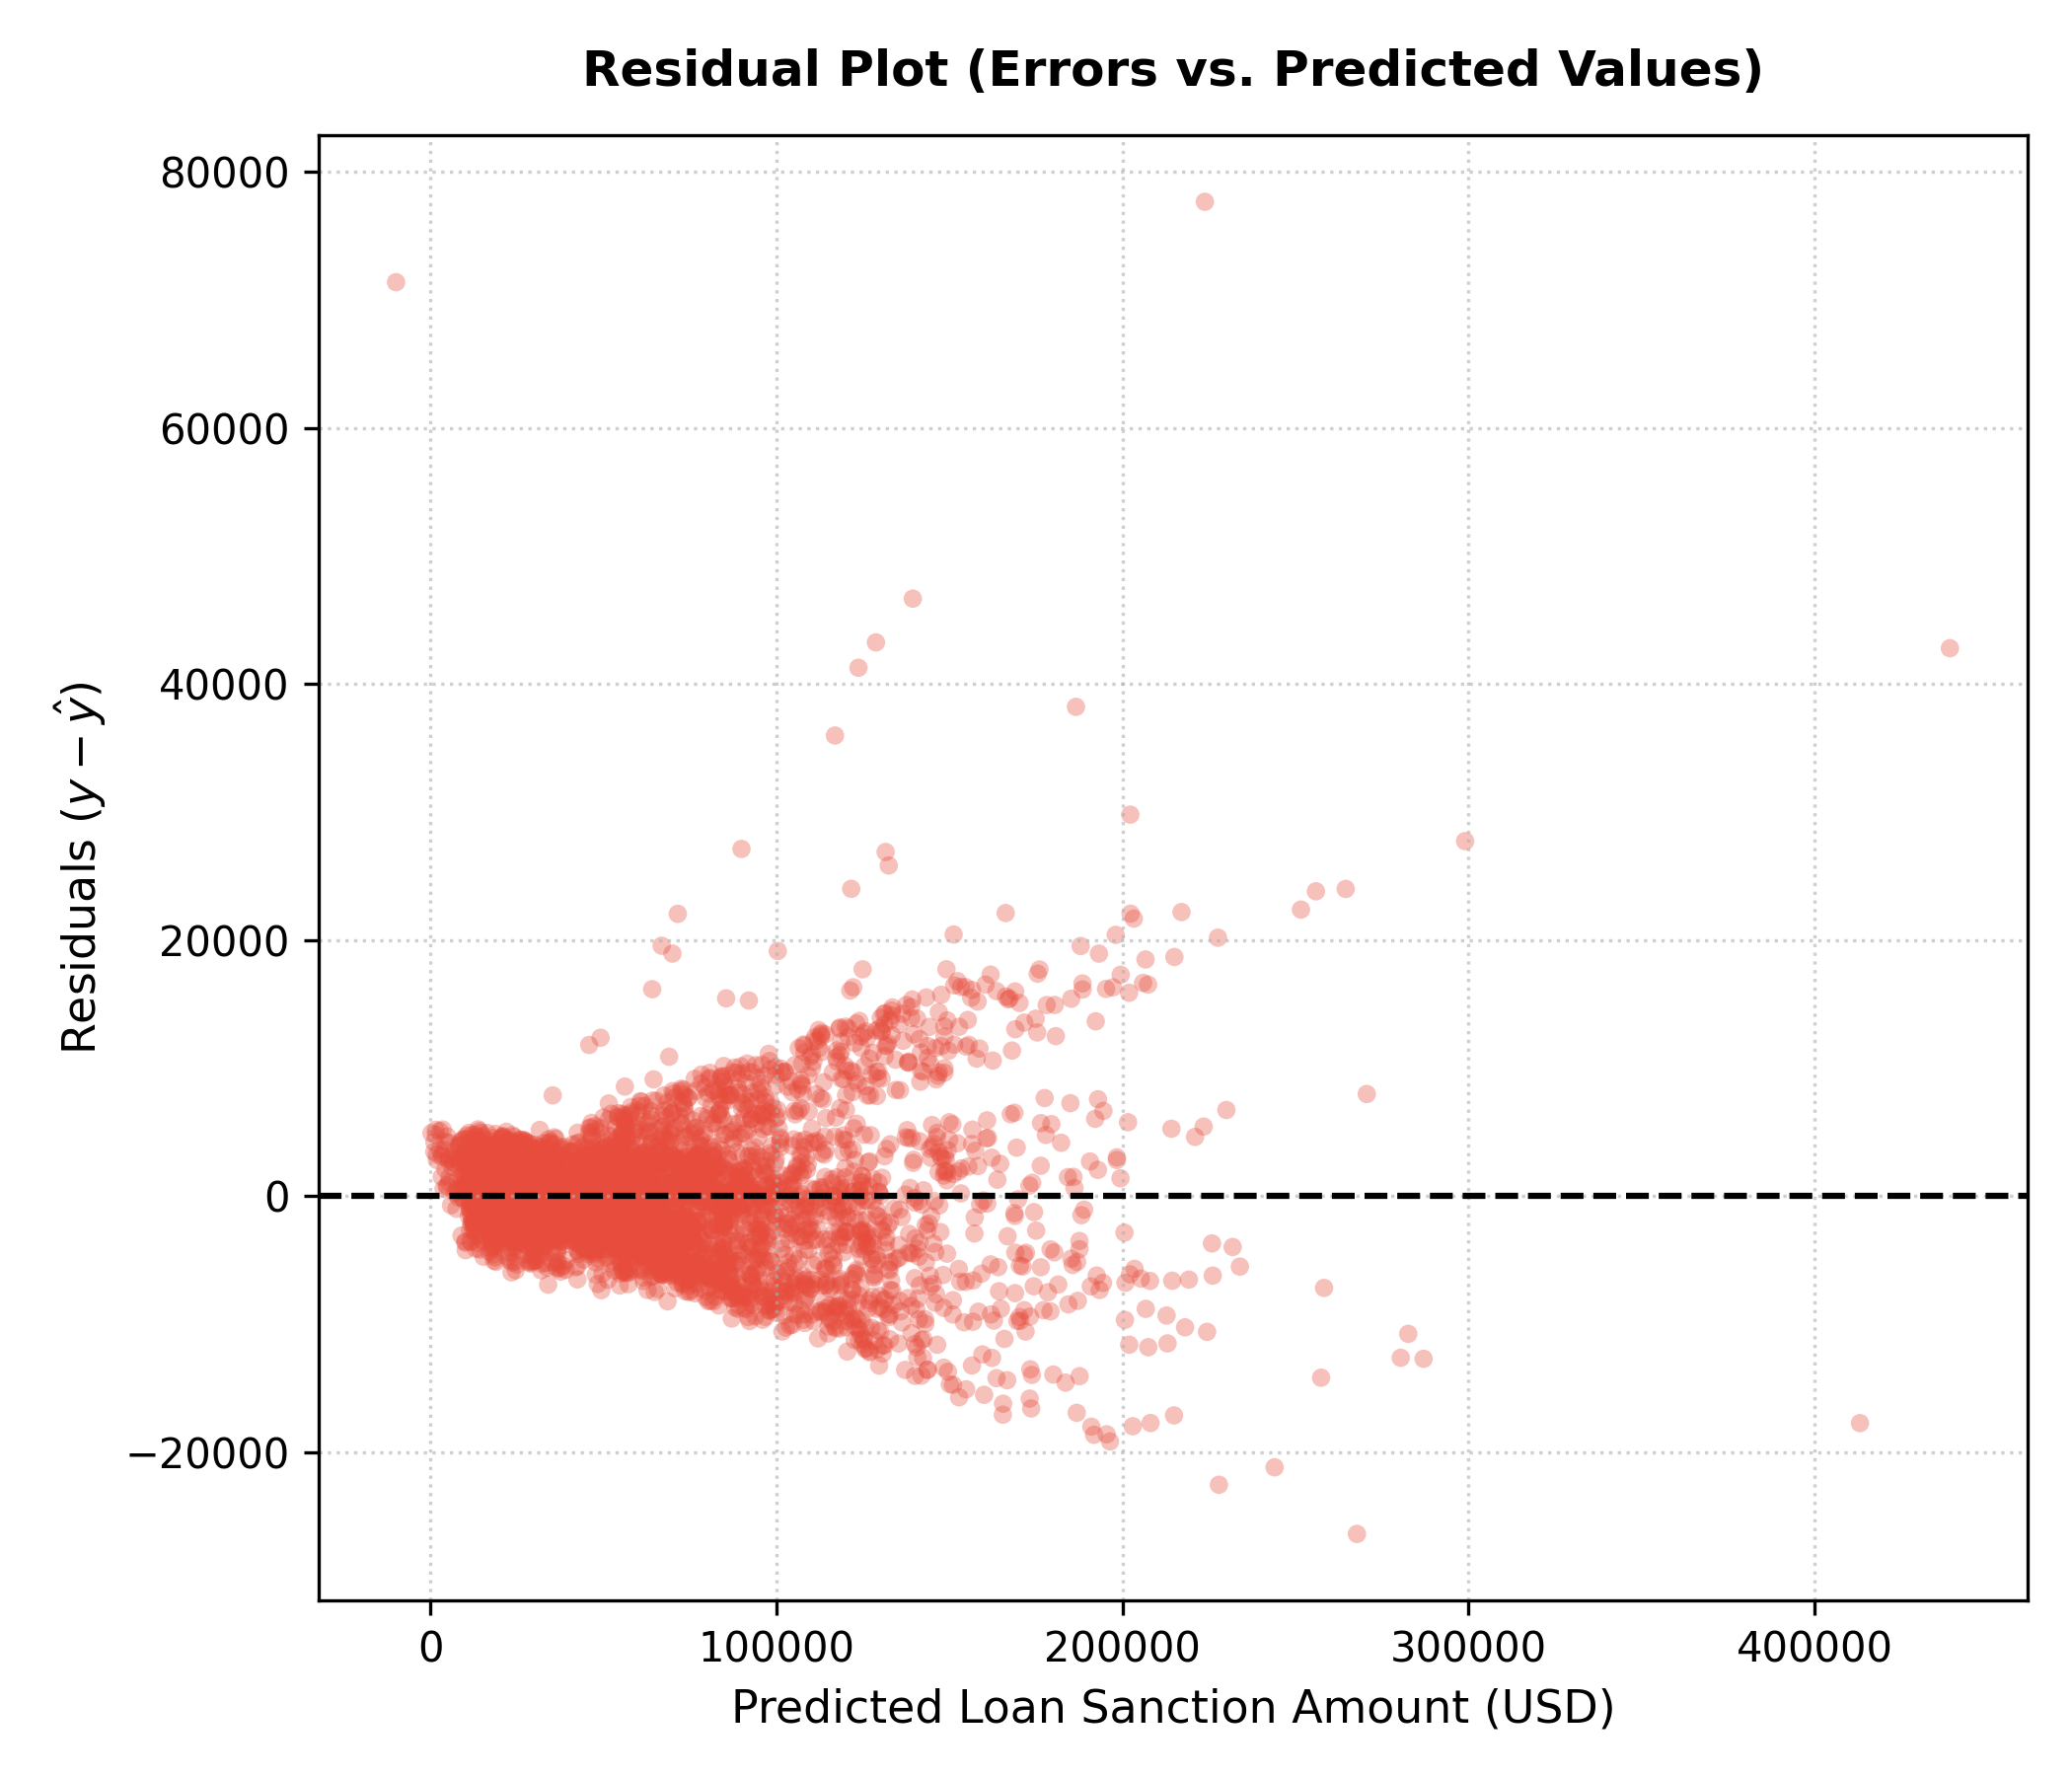
\includegraphics[width=0.65\linewidth]{figures/residual_plot.png}
\caption{Residual Plot (Prediction Errors vs. Predicted Values)}
\label{fig:residuals}
\vspace{0.2cm}
\small
\textbf{Inference:}
Residual errors scatter symmetrically around the zero horizon line ($y=0$). The absence of heteroscedastic fan patterns or non-linear trends confirms constant error variance and validates linear model assumptions.
\end{minipage}
\end{figure}

\begin{figure}[!htbp]
\centering
\begin{minipage}{\linewidth}
\centering
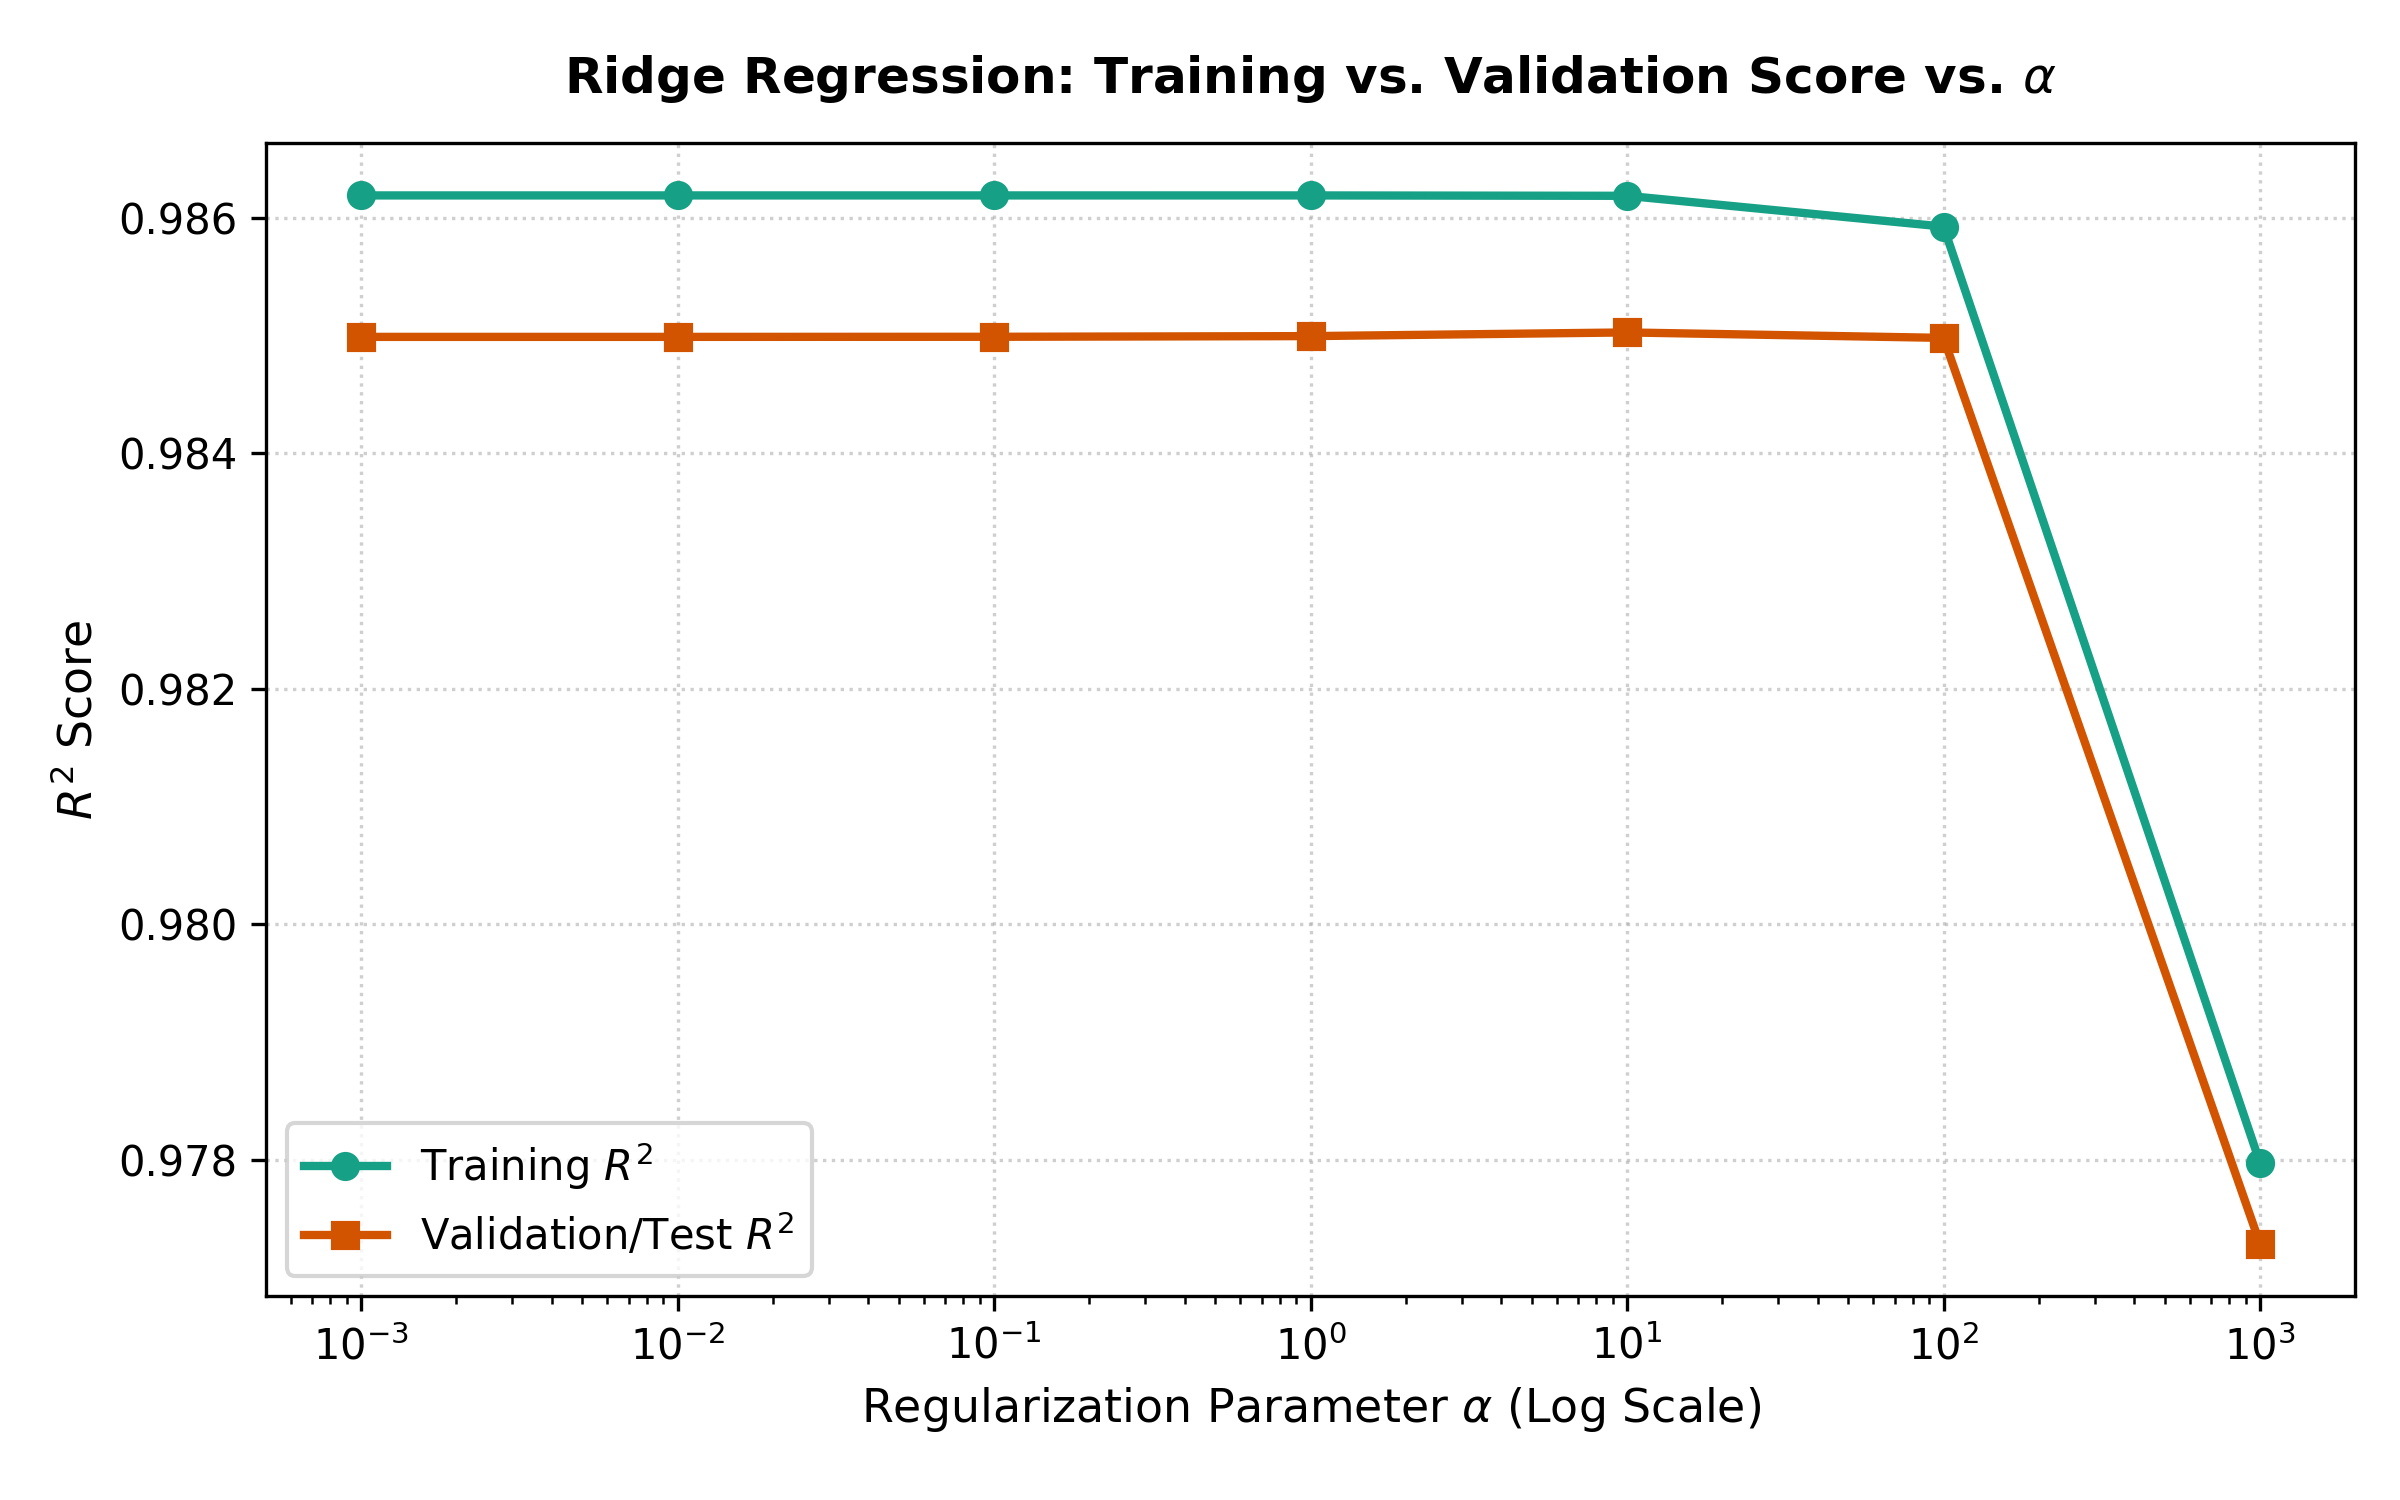
\includegraphics[width=0.72\linewidth]{figures/train_vs_val_error.png}
\caption{Ridge Regression: Training vs. Validation $R^2$ vs. Regularization Strength ($\alpha$)}
\label{fig:train_val_r2}
\vspace{0.2cm}
\small
\textbf{Inference:}
Validation curves demonstrate stable training and validation $R^2$ performance across $\alpha \in [10^{-3}, 1.0]$. As regularization strength exceeds $\alpha > 10.0$, validation performance degrades rapidly due to excessive shrinkage, indicating underfitting.
\end{minipage}
\end{figure}

\section{Overfitting and Underfitting Analysis}

\begin{itemize}
    \item \textbf{Difference Between Training and Validation Errors:} Unregularized OLS achieves $R^2 = 0.9850$ on test data, whereas tuned Lasso reaches $R^2 = 0.9856$. The minimal gap between training and evaluation scores indicates low risk of overfitting on the scaled feature space.
    \item \textbf{Effect of Regularization Strength ($\alpha$):} Small values ($\alpha \le 0.1$) perform identically to OLS. Optimal penalty strength ($\alpha = 10.0$ for Lasso, $\alpha = 1.0$ for Ridge) balances model complexity and generalization. Large values ($\alpha \ge 100.0$) lead to severe underfitting.
    \item \textbf{Improvement in Generalization After Tuning:} 5-Fold Cross-Validation optimization identified optimal regularizer hyperparameters, improving test $R^2$ to 0.9856 and reducing RMSE by over \$110 compared to baseline linear regression.
\end{itemize}

\section{Bias--Variance Analysis}

\begin{itemize}
    \item \textbf{Bias Behavior of Linear Regression:} Baseline OLS demonstrates low systematic bias due to the pronounced linear correlation between requested amounts, collateral valuations, credit scores, and sanctioned loan limits.
    \item \textbf{Variance Reduction in Ridge and Elastic Net:} $L_2$ shrinkage in Ridge smoothly constrains correlated feature weights, mitigating variance inflation caused by multicollinearity.
    \item \textbf{Feature Sparsity Effect in Lasso:} $L_1$ regularization in Lasso sets non-essential predictor coefficients to zero, creating a sparse, highly interpretable model structure without sacrificing predictive accuracy.
\end{itemize}

\section{Observations and Conclusion}
In this experiment, Linear Regression, Ridge, Lasso, and Elastic Net models were implemented and evaluated on the loan sanction dataset following the 9 mandated steps. Rigorous data preprocessing (median/mode imputation, one-hot encoding, and standard scaling) established a clean pipeline. Hyperparameter tuning using 5-Fold Cross-Validation identified optimal regularized models (Lasso $\alpha=10.0$, Ridge $\alpha=1.0$), achieving a top test accuracy of $R^2 = 0.9856$ and RMSE = \$5,504.23. The regularized models effectively controlled variance, eliminated uninformative predictors, and demonstrated robust generalization performance over baseline OLS regression.

\section{References}
\begin{enumerate}[label={[\arabic*]}, leftmargin=2em]
    \item Scikit-learn Documentation, ``Linear Models,'' \url{https://scikit-learn.org/stable/modules/linear_model.html}.
    \item Scikit-learn Documentation, ``Hyperparameter Tuning with GridSearchCV,'' \url{https://scikit-learn.org/stable/modules/grid_search.html}.
    \item A. Géron, \textit{Hands-On Machine Learning with Scikit-Learn, Keras, and TensorFlow}, 3rd ed., O'Reilly Media, 2022.
    \item Kaggle Repository, ``Predict Loan Amount Data,'' \url{https://www.kaggle.com/datasets}.
\end{enumerate}

\end{document}
